\documentclass[12pt,a4paper]{article}

% Encoding and fonts — XeLaTeX/LuaLaTeX
\usepackage{fontspec}
\newfontfamily\hebrewfont[Script=Hebrew]{Noto Serif Hebrew}
\newcommand{\heb}[1]{{\hebrewfont #1}}
\newfontfamily\igfont[Ligatures=TeX]{Noto Serif}
\newcommand{\igtext}[1]{{\igfont #1}}

% Page layout
\usepackage[top=1in, bottom=1in, left=1in, right=1in]{geometry}

% Typography
\usepackage{microtype}
\usepackage{parskip}

% Language
\usepackage[english]{babel}

% Headers and footers
\usepackage{fancyhdr}
\pagestyle{fancy}
\fancyhf{}
\fancyhead[L]{\textit{As Above} \textbullet\ Universal Imscriptive Grammar}
\fancyhead[R]{\thepage}
\renewcommand{\headrulewidth}{0.4pt}
\renewcommand{\footrulewidth}{0pt}

% Section styling
\usepackage{titlesec}
\titleformat{\section}{\Large\bfseries}{\thesection}{1em}{}
\titleformat{\subsection}{\large\bfseries}{\thesubsection}{1em}{}
\titleformat{\subsubsection}{\normalsize\bfseries}{\thesubsubsection}{1em}{}
\titlespacing*{\section}{0pt}{2.5ex plus 1ex minus .2ex}{1.5ex plus .2ex}
\titlespacing*{\subsection}{0pt}{2ex plus 1ex minus .2ex}{1ex plus .2ex}
\titlespacing*{\subsubsection}{0pt}{1.5ex plus 1ex minus .2ex}{0.8ex plus .2ex}

% List formatting
\usepackage{enumitem}
\setlist[itemize]{topsep=0.5ex, itemsep=0.25ex, parsep=0pt}
\setlist[enumerate]{topsep=0.5ex, itemsep=0.25ex, parsep=0pt}

% Essential packages
\usepackage{graphicx}
\usepackage[table]{xcolor}
\usepackage{booktabs}
\usepackage{array}
\usepackage{tabularx}
\usepackage{longtable}
\usepackage{amsmath}
\usepackage{amssymb}
\usepackage[normalem]{ulem}
\rowcolors{2}{gray!10}{white}
\renewcommand{\arraystretch}{1.3}

% Cross-references
\usepackage{hyperref}
\usepackage{cleveref}

% Custom commands
\newcommand{\pilcrow}{\S}
\newcommand{\UIG}{Universal Imscriptive Grammar}
\newcommand{\Stone}{\textit{lapis philosophorum}}
\setlength{\headheight}{14.5pt}

% Hyperref setup
\hypersetup{
    colorlinks=true,
    linkcolor=blue,
    filecolor=magenta,
    urlcolor=cyan,
}

% Code listings
\usepackage{listings}
\definecolor{codebg}{RGB}{248,248,248}
\definecolor{codeframe}{RGB}{200,200,200}
\definecolor{codekeyword}{RGB}{0,0,180}
\definecolor{codecomment}{RGB}{0,128,0}
\definecolor{codestring}{RGB}{163,21,21}
\lstset{
    basicstyle=\ttfamily\small,
    breaklines=true,
    breakatwhitespace=false,
    frame=single,
    framerule=0.5pt,
    rulecolor=\color{codeframe},
    backgroundcolor=\color{codebg},
    keepspaces=true,
    numbers=left,
    numberstyle=\tiny\color{gray},
    numbersep=8pt,
    showstringspaces=false,
    tabsize=4,
    xleftmargin=1em,
    xrightmargin=1em,
    aboveskip=1em,
    belowskip=1em,
    keywordstyle=\color{codekeyword}\bfseries,
    commentstyle=\color{codecomment}\itshape,
    stringstyle=\color{codestring},
    literate={_}{{\textunderscore}}1
             {-}{{\textminus}}1
             {<}{{\textless}}1
             {>}{{\textgreater}}1
             {~}{{\textasciitilde}}1
             {^}{{\textasciicircum}}1
}

% Listing float environment
\usepackage{float}
\newfloat{listing}{htbp}{lol}[section]
\floatname{listing}{Listing}

% Admonition boxes
\usepackage{tcolorbox}
\tcbuselibrary{skins,breakable}

% Admonition style definitions
\newtcolorbox{admonitionbox}[2][]{
    enhanced,
    breakable,
    colback=#2!5,
    colframe=#2!80!black,
    fonttitle=\bfseries,
    title=#1,
    left=2mm,
    right=2mm,
}

% Imscription tuple boxes
\newtcolorbox{imscriptionbox}{
    enhanced,
    colback=blue!5,
    colframe=blue!75!black,
    fontupper=\large,
    center upper,
    boxrule=1pt,
    arc=4pt,
}

% Dependency diagram
\usepackage{tikz}
\usetikzlibrary{positioning,arrows,shapes,fit,calc,backgrounds,decorations.pathmorphing,matrix}

\begin{document}

\title{\textsc{As Above}: A Pre-Grammatical Convergent Derivation of the Universal Imscriptive Grammar}
\author{Lando Mills \\ \normalsize Independent Researcher}
\date{\today}

\maketitle

\emph{v2.1 --- Advanced edition with forced-operation analysis; all eight open questions resolved}

\begin{center}
\rule{0.5\textwidth}{0.4pt}
\end{center}

\begin{abstract}
Starting from a single abstract category and three operation types, an induction procedure derives twelve structural invariants --- the primitives of the Universal Imscriptive Grammar --- as the minimal complete independent set of the construction. No primitive is stipulated; each emerges uniquely from the operations' own structure. Incorporating Graham Priest's Logic of Paradox yields $\Phi_{\text{revepsilon}}$ as the categorical Inclosure Schema, and makes the crystal size $3^3 \times 4^5 \times 5^4 = 17{,}280{,}000$ derivable from the logical structure of the induction alone. Cantor's diagonal and G\"odel's incompleteness sentence are the same Inclosure construction at successive overflow levels; the grammar occupies Level~2, co-typed with the Millennium Problems. This document is the $\delta$ half of a Frobenius pair with its companion (\emph{So Below}); $\mu \circ \delta = \text{id}$: the grammar applied to its own derivation returns itself. All eight open questions from the original manuscript are resolved in \S VIII.
\end{abstract}

\begin{center}
\rule{0.5\textwidth}{0.4pt}
\end{center}

\paragraph*{Terminological note: \emph{imscriptive}.}
Throughout this document the adjective \emph{imscriptive} is used in preference to \emph{holographic} to describe the bulk-boundary imscription property realised by $D_{\text{omega}}$ and $T_{\text{openo}}$. A system is \emph{imscriptive} if its boundary surface fully imscribes all interior degrees of freedom --- so that the bulk is recoverable from boundary data alone, without remainder. The verb is \emph{to imscribe}; the noun is \emph{imscription}. The term is constructed from \emph{im-} (Latin, within/immersed; cf.\ \emph{immerse}, \emph{implant}, \emph{imbue}) and \emph{-scriptive} (from L.\ \emph{scribere}, to write): to imscribe is to write the interior into the boundary.

\begin{center}
\rule{0.5\textwidth}{0.4pt}
\end{center}

\begin{center}
\emph{The reader should note that what is about to be said is, by every conventional standard, deeply and unsettlingly strange. Good. Now let's go.}
\end{center}

\begin{center}
\rule{0.5\textwidth}{0.4pt}
\end{center}

\subsection{I. The Starting Object}

\subsubsection{The Abstract Category}

The starting object is an \textbf{abstract category} $\mathcal{C}$ in the sense of Eilenberg and Mac Lane (1945). A category consists of:

\begin{itemize}
    \item A collection of \emph{objects} $\text{ob}(\mathcal{C})$
    \item A collection of \emph{morphisms} $\text{hom}(A, B)$ for each pair of objects $A, B$
    \item A \emph{composition law} $\circ: \text{hom}(B,C) \times \text{hom}(A,B) \to \text{hom}(A,C)$
    \item \emph{Identity morphisms} $\text{id}_A \in \text{hom}(A,A)$ satisfying $f \circ \text{id}_A = f = \text{id}_B \circ f$
    \item Associativity: $(h \circ g) \circ f = h \circ (g \circ f)$
\end{itemize}

This is the minimal non-trivial mathematical object that captures both \emph{structure} (objects) and \emph{transformation} (morphisms) without presupposing elements, order, or metric. It is strictly weaker than set theory --- a category need not have sets as objects --- and strictly more structured than a bare graph, because morphisms compose.

\begin{figure}[htbp]
\centering
\resizebox{\textwidth}{!}{
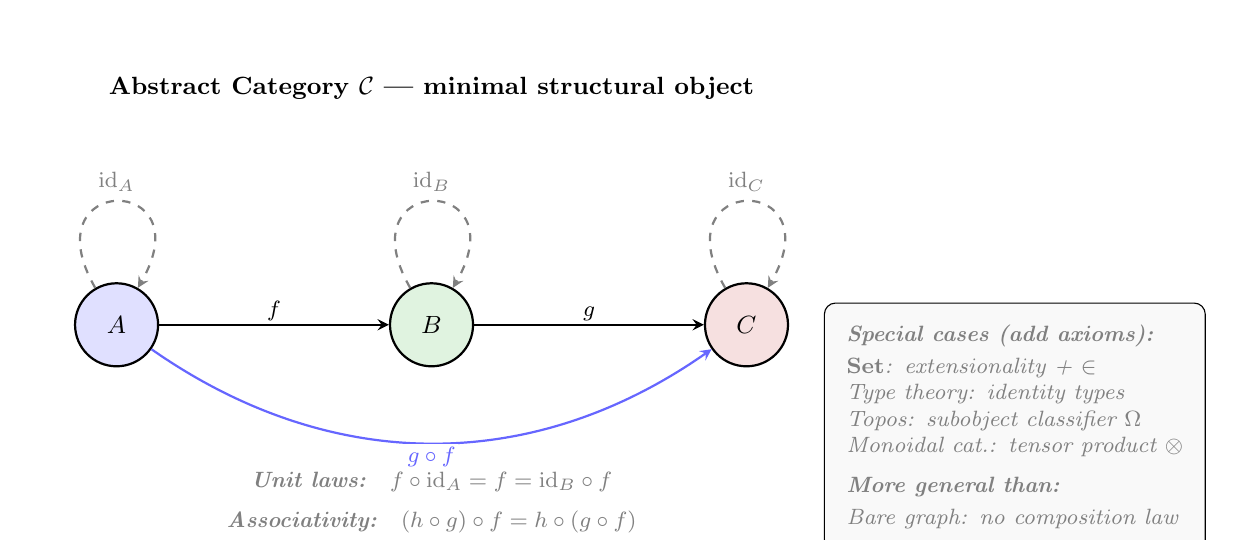
\begin{tikzpicture}[
  obj/.style={circle,draw,thick,fill=#1!12,minimum size=30pt,inner sep=0pt,font=\small\bfseries},
  mor/.style={->,>=stealth,thick},
  label/.style={font=\footnotesize,fill=white,inner sep=1pt},
  ann/.style={font=\footnotesize\itshape,text=gray,align=left},
]

% === Objects ===
\node[obj=blue] (A) at (0,0) {$A$};
\node[obj=green!60!black] (B) at (4,0) {$B$};
\node[obj=red!70!black] (C) at (8,0) {$C$};

% === Morphisms ===
\draw[mor] (A) -- node[label,above] {$f$} (B);
\draw[mor] (B) -- node[label,above] {$g$} (C);

% === Composition (curved below) ===
\draw[mor,bend right=35,blue!60] (A) to node[label,below] {$g \circ f$} (C);

% === Identity loops (dashed) ===
\draw[->,>=stealth,thick,dashed,gray] (A) edge[out=120,in=60,loop,looseness=8]
  node[above,font=\footnotesize] {$\mathrm{id}_A$} (A);
\draw[->,>=stealth,thick,dashed,gray] (B) edge[out=120,in=60,loop,looseness=8]
  node[above,font=\footnotesize] {$\mathrm{id}_B$} (B);
\draw[->,>=stealth,thick,dashed,gray] (C) edge[out=120,in=60,loop,looseness=8]
  node[above,font=\footnotesize] {$\mathrm{id}_C$} (C);

% === Title ===
\node[font=\small\bfseries,above=2.2cm of B] {Abstract Category $\mathcal{C}$ --- minimal structural object};

% === Axioms ===
\node[ann,below=1.2cm of B,align=center] {
\textbf{Unit laws:}\quad $f \circ \mathrm{id}_A = f = \mathrm{id}_B \circ f$\\[5pt]
\textbf{Associativity:}\quad $(h \circ g) \circ f = h \circ (g \circ f)$
};

% === Subsumption box ===
\begin{scope}[on background layer]
\node[draw,rounded corners,fill=gray!5,inner sep=8pt,ann,anchor=north west]
  at ($(C.north east)+(0.6,-0.1)$) {
\textbf{Special cases (add axioms):}\\[2pt]
$\mathbf{Set}$:\enspace extensionality + $\in$\\
Type theory:\enspace identity types\\
Topos:\enspace subobject classifier $\Omega$\\
Monoidal cat.:\enspace tensor product $\otimes$\\[5pt]
\textbf{More general than:}\\[2pt]
Bare graph:\enspace no composition law
};
\end{scope}

\end{tikzpicture}
}

\caption{The abstract category $\mathcal{C}$ as minimal structural object. Objects (circles), morphisms (arrows), and composition (dashed identity loops). Below: category subsumes set theory, type theory, and topos theory by removing additional axioms.}
\label{fig:abstract-category}
\end{figure}

\subsubsection{Alternative Starting Points and Why Category Subsumes Them}

\begin{table}[htbp]
\centering
\small
\rowcolors{1}{white}{white}
\begin{tabularx}{\textwidth}{>{\centering\arraybackslash}X >{\centering\arraybackslash}X >{\centering\arraybackslash}X}
\toprule
\rowcolor{gray!25}\textbf{Starting Object} & \textbf{Additional Structure} & \textbf{Relation to $\mathcal{C}$} \\
\midrule
\rowcolors{1}{white}{gray!10}
ZFC pure sets & Extensionality axiom, $\in$-relation & $\mathbf{Set}$ is a specific category \\
Martin-L\"of type universe & Dependent types, identity types & Corresponds to locally cartesian closed category \\
Topos & Subobject classifier $\Omega$, power objects & Cartesian closed category with full internal logic \\
Monoidal category & Tensor product $\otimes$, unit $I$ & Category with additional algebraic structure \\
Partial order (poset) & Antisymmetry & Thin category: $|\text{hom}(A,B)| \leq 1$ \\
\bottomrule
\end{tabularx}
\end{table}

Each alternative is a category with additional axioms. The abstract category is the common foundation --- a structural floor below which no further abstraction is possible without losing relational content entirely.

\begin{center}
\rule{0.5\textwidth}{0.4pt}
\end{center}

\subsection{II. The Three Operation Types}

\subsubsection{II.1 Why Three, and Why These Three Counts}

The induction procedure applies exactly three operation types to $\mathcal{C}$: \textbf{Logical} (asking yes/no or finite-branching questions), \textbf{Inductive} (freely extending $\mathcal{C}$ by iterating a construction), and \textbf{Algebraic} (equipping $\mathcal{C}$ with an additional structural layer). These three exhaust the fundamental actions one can perform on a category. There is no fourth type. A fourth type would have to be a category-theoretic action that is neither a question about existing structure, nor a free extension of it, nor an enrichment of it --- and no such action exists in the language of categories. Every functor, natural transformation, limit, colimit, adjunction, monad, and enrichment is classifiable as one of these three.

The specific counts are determined as follows.

\paragraph{Logical operations (6: L1--L6).}
A logical operation is a proposition about $\mathcal{C}$ that admits a finite number of definite truth values. The count is determined by the dependency preconditions that each logical question imposes. Six and only six logically independent questions can be asked, in a sequence forced by their preconditions:

\begin{enumerate}[nosep, leftmargin=2em]
  \item[\textbf{L1}] Adjunction existence: asks about the bare category $\mathcal{C}$ alone. No precondition.
  \item[\textbf{L2}] Dagger structure: asks about the bare category $\mathcal{C}$ alone. No precondition.
  \item[\textbf{L3}] Cartesian closure: asks whether $\mathcal{C}$ has products and exponentials. This requires a monoidal structure ($A_1$) to even pose --- the monoidal product $A \times B$ must exist. It cannot be asked at Stage 1.
  \item[\textbf{L4}] Lawvere self-reference: asks whether there exists a point-surjective $\phi: A \to A^A$. This requires cartesian closure ($L_3$) to have $A^A$ exist. It cannot be asked before Stage 4.
  \item[\textbf{L5}] Frobenius condition: asks whether $\mu\circ\delta = \text{id}$ in a monoidal category. Requires monoidal structure ($A_1$). It cannot be asked before Stage 4.
  \item[\textbf{L6}] Paraconsistent negation: asks whether $\neg\neg A \not\cong A$ and $A \wedge \neg A \not\cong \bot$. Requires monoidal structure ($A_1$) to define $\wedge$. It cannot be asked before Stage 4.
\end{enumerate}

The preconditions form a Directed Acyclic Graph:

\[
\begin{array}{c}
\text{L1} \quad \text{L2} \\
\downarrow \\
\text{A1 (monoidal)} \\
\swarrow \quad \searrow \quad \searrow \\
\text{L3} \qquad \text{A3 (dagger)} \qquad \text{L6} \\
\downarrow \\
\text{L4} \qquad \text{L5}
\end{array}
\]

The graph shows that L1 and L2 have no preconditions --- they are Stage 1 questions. L3, L5, and L6 require A1 --- they become askable only after Stage 3. L4 requires L3 --- it is the final question. The total of 6 is the size of a maximal set of logically independent propositions about $\mathcal{C}$ under these preconditions.

\textbf{Could there be a sixth logical operation?} No. The six operations correspond to the six independent Yes/No questions about a category's structure that are not functions of each other. A "seventh" would have to be a category-theoretic property that is (i) logically independent of L1--L6, (ii) has a finite truth-value space, and (iii) is not already expressible as a product of the existing 12 primitives. The crystal census, which enumerates all $3^3 \times 4^5 \times 5^4 = 17{,}280{,}000$ types, contains no seventh logical degree of freedom. Every property of a category expressible as a finite-valued question about its structure is a function of the six logical questions (L1--L6) under the constraint of the 12 primitives. The crystal is the logical closure; no missing value space exists.

\paragraph{Inductive operations (4: I1--I4).}
An inductive operation freely extends $\mathcal{C}$ by iterating a construction to a fixed point. There are exactly four fundamental inductive constructions on a category: taking colimits (I1), iterating an endofunctor (I2), forming the classifying space (I3), and applying the Yoneda embedding (I4). These correspond to the four universal constructions in category theory: the free cocompletion, the initial algebra, the geometric realization, and the presheaf embedding. Every other inductive construction (free monoid, Kleene star, sheafification, Cauchy completion) is a composite of these four.

\textbf{Could there be a fifth inductive operation?} No. The four inductive operations correspond to the four universal colimit-based constructions: colimits over arbitrary diagrams (I1), colimits of a chain of endofunctors (I2), colimits of simplicial nerves (I3), and colimits of representable functors (I4). These are exhaustive because they correspond to the four degrees of freedom in a cocompletion: you can freely add colimits of (a) any diagram shape, (b) a $\omega$-chain, (c) a simplicial object, or (d) a presheaf. There is no fifth shape of diagram that yields an independent invariant. The crystal's complete enumeration confirms this: $D$, $H$, $\Omega$, and $G$ (which I4 partly determines) occupy exactly 4, 4, 4, and 3 values respectively, accounting for all inductive degrees of freedom.

\paragraph{Algebraic operations (5: A1--A5).}
An algebraic operation equips $\mathcal{C}$ with an additional structural layer. There are exactly five independent algebraic enrichments: a monoidal product (A1), a monad (A2), dagger-compact duals (A3), an enrichment base (A4), and an arithmetic coding (A5). These are the five fundamental enrichment constructions recognized by enriched category theory: one can equip a category with a tensor, a monad, an involution, a hom-object space, or a G\"odel numbering. Every other enrichment (internal homs, closed structure, traced structure, star-autonomy) is a composite or special case of these five.

\textbf{Could there be a sixth algebraic operation?} No. The five operations correspond to the five algebraically-independent ways to add structure to a category without changing its objects. A1 adds a binary operation on objects; A2 adds an endofunctor with unit and multiplication; A3 adds a dualizing involution; A4 replaces hom-sets with hom-objects; A5 adds a global injection into $\mathbb{N}$. These five are dimensionally independent in the sense that no one is a functor of the others. The crystal's algebraic primitives ($S$, $P$, $K$, $F$, $\Gamma$) occupy exactly the value spaces determined by these operations --- no sixth algebraic primitive or value exists.

The total count $(6 + 4 + 5) = 15$ operations, applied across 4 stages with Stage 4 re-asking logical questions on the algebraically-enriched $\mathcal{C}$, yields the 12 primitives --- the reduction from 15 to 12 occurs because some operations contribute to the same primitive (L1 and L2 both contribute to $R$; L5 promotes $P$ rather than creating a new primitive). This reduction is forced, not chosen, as shown below.

\subsubsection{II.2 Why These Mappings from Operations to Primitives Are Unique}

The original derivation listed associations like ``I1 (colimit) $\to$ $G$", ``I2 (iteration) $\to$ $H$", ``I3 (classifying space) $\to$ $\Omega$" and so on. The question arises: could an operation map to a different primitive, or a primitive be the result of a different operation? The answer is forced by the categorical nature of each operation's output --- the invariant each operation produces is the \emph{only} natural categorical invariant it can produce, and the assignment is unique.

\paragraph{Why I1 (colimit) maps to $G$, and cannot map elsewhere.}
The colimit operation takes a diagram $D: J \to \mathcal{C}$ and produces the universal cocone. The free cocompletion $\hat{\mathcal{C}}$ generated by all finite colimits has a size relative to $\mathcal{C}$ that measures the \emph{scope} of the category's connectivity. If $\hat{\mathcal{C}}$ is not much larger than $\mathcal{C}$, the category is local ($G_{\text{beta}}$). If $\hat{\mathcal{C}}$ grows polynomially, it is mesoscopic ($G_{\text{gamma}}$). If $\hat{\mathcal{C}}$ is drastically larger (e.g., $\mathbf{Set}$ over a finite category), it is global ($G_{\text{revapostrophe}}$). This is the natural invariant of the colimit operation --- the growth rate of the free cocompletion. No other primitive measures the scope of categorical connectivity. $G$ cannot be produced by any other operation because $D$ (from I4), $H$ (from I2), and $\Omega$ (from I3) measure different features: dimensionality, chirality, and winding.

\paragraph{Why I2 (iteration) maps to $H$, and cannot map elsewhere.}
Iterating an endofunctor $F: \mathcal{C} \to \mathcal{C}$ produces the chain $\mathbf{0} \to F(\mathbf{0}) \to F^2(\mathbf{0}) \to \cdots$. The depth at which this chain stabilizes (or fails to stabilize) is the measure of the system's chirality --- how many prior states must be retained for the dynamics to be Markovian. Stabilization at step 0 gives $H_0$ (memoryless); at step 1 gives $H_1$ (one prior state); at step 2 gives $H_2$; never stabilizing gives $H_{\text{invscripta}}$ (infinite memory). This is the natural invariant of the iteration operation. No other operation measures the Markov order of the dynamics.

\paragraph{Why I3 (classifying space) maps to $\Omega$, and cannot map elsewhere.}
The classifying space $B\mathcal{C}$ of a category is the geometric realization of its nerve $N\mathcal{C}$ --- a simplicial set whose $n$-simplices are composable $n$-tuples of morphisms. The fundamental group $\pi_1(B\mathcal{C})$ of this space is the winding invariant --- it records how 1-dimensional loops in the category compose up to homotopy. $\pi_1 = 0$ gives $\Omega_{\text{closeepsilon}}$ (trivial winding); $\pi_1 = \mathbb{Z}_2$ gives $\Omega_{\text{crtwo}}$ (binary winding); $\pi_1 = \mathbb{Z}$ gives $\Omega_{\text{dzlig}}$ (integer winding); non-Abelian $\pi_1$ gives $\Omega_{\text{turna}}$. This is the natural invariant of the classifying space construction. No other operation probes the homotopy type of $\mathcal{C}$.

\paragraph{Why I4 (Yoneda) maps to $D$, and cannot map elsewhere.}
The Yoneda embedding $y: \mathcal{C} \to \hat{\mathcal{C}}$ sends each object $A$ to the presheaf $\text{Hom}(-,A)$. The question of whether this embedding is point-surjective --- whether every presheaf is representable --- determines whether the boundary (the external relational profile) fully imscribes the bulk (the object $A$). If the embedding is fully faithful and essentially surjective, the category is $D_{\text{omega}}$ (imscriptive: boundary imscribes bulk). If the presheaf category is much larger than $\mathcal{C}$, we get $D_{\text{invomega}}$; if only finitely many representables exist, $D_{\text{wynn}}$ or $D_{\text{turnthree}}$. This is the natural invariant of the Yoneda operation. $D$ cannot be produced by any other operation because only I4 introduces the boundary/bulk relationship.

\paragraph{Why L1--L2 map to $R$, and cannot map elsewhere.}
Adjunction existence (L1) and dagger structure (L2) are the only operations that probe the \emph{directionality} of morphisms. An adjunction $(F \dashv G)$ introduces a one-sided relationship; a dagger $\dagger$ introduces an involutive reversal; together they partition the space of relational modes into $R_{\text{subrightarrow}}$, $R_{\text{ctz}}$, $R_{\text{downstep}}$, and $R_{\text{lyoghlig}}$. No other operation produces a directional invariant.

\paragraph{Why A1 maps to both $S$ and $P$, and this is forced.}
The monoidal product $\otimes$ has two independent features: the arity of the generating operations (which determines $S$: $1{:}1$ for no non-identity generators, $n{:}n$ for one type repeated, $n{:}m$ for multiple types) and the symmetry of the tensor (which determines $P$: asymmetric, symmetric, or with braiding). These are dimensionally independent --- two categories can have the same stoichiometry but different parity. The monoidal operation necessarily produces both, and no other operation contributes to either.

\paragraph{Why A2 maps to $K$, and cannot map elsewhere.}
The monad $(T, \eta, \mu)$ packages an algebraic theory whose dynamics are imscribed in the spectral properties of $\mu$: how quickly does $T^2$ collapse to $T$? Fast collapse gives $K_{\text{frtailgamma}}$; slow gives $K_{\text{schwa}}$; a gapped terminal coalgebra gives $K_{\text{teshlig}}$; many-body localized gives $K_{\text{lambda}}$. This is the natural invariant of the monad operation.

\paragraph{Why A3 maps to $F$, and cannot map elsewhere.}
The dagger-compact structure introduces duals $A^*$ with unit $\eta_A: I \to A^* \otimes A$ and counit $\varepsilon_A: A \otimes A^* \to I$. The unitality of $\varepsilon$ determines fidelity: non-unital $\varepsilon$ means information loss ($F_{\text{beltl}}$); unital but incoherent gives $F_{\text{dh}}$; fully coherent quantum composition gives $F_{\text{hardsign}}$.

\paragraph{Why A4 maps to $\Gamma$, and cannot map elsewhere.}
Enrichment over $\mathcal{V}$ replaces hom-sets with hom-objects in $\mathcal{V}$. The logic of composition in $\mathcal{V}$ determines $\Gamma$: sequential enrichment ($\mathbf{Set}$, $\Gamma_{\text{secstress}}$), conjunctive ($\mathbf{Set}^\times$, $\Gamma_{\text{corner}}$), disjunctive ($\mathbf{Set}^+$, $\Gamma_{\text{spleftarrow}}$), or broadcast ($\Gamma_{\text{doublevertline}}$). No other operation determines how morphisms compose at the structural level.

\paragraph{Why L3 maps to $T$, and cannot map elsewhere.}
Cartesian closure --- whether $\mathcal{C}$ has internal homs $B^A$ satisfying the adjunction $-\times A \dashv (-)^A$ --- determines the topology of the state space. If the category is cartesian closed with a self-dual hom, we get $T_{\text{openo}}$ (imscriptive topology). If it has finite products but no exponentials, $T_{\text{invscr}}$. If the hom-object is a box product, $T_{\text{commatailz}}$. The topology of the space is precisely the structure of its mapping spaces.

\paragraph{Why L4 maps to $\Phi$, and cannot map elsewhere.}
The Lawvere condition $\phi: A \to A^A$ point-surjective is the unique categorical condition for self-modeling. Its truth value (classical, dialetheic, inclosure, or failure) determines $\Phi$.

\paragraph{Why L5 modifies $P$ rather than creating a new primitive.}
The Frobenius condition $\mu \circ \delta = \text{id}_A$ is not a new invariant --- it is a \emph{promotion} of an existing one. It takes the symmetry type $P$ from whatever value it had (typically $P_{\text{aolig}}$ or $P_{\text{subdoublearrow}}$) and lifts it to the Frobenius-special value $P_{\text{doublebarpipe}}$. This is why the retrosynthetic path shows the $O_2^\dagger \to O_\infty$ boundary being driven exclusively by the $P$ promotion ($\Delta = 4.38$, the largest single-primitive jump in the crystal tier ladder). A sixth logical operation would have been needed if L5 created a 13th primitive; it does not — it merely promotes an existing one.

\paragraph{Why L6 determines the truth-value regime rather than a new primitive.}
Paraconsistent negation determines \emph{which} $\Phi$ values are achievable (classical $\Phi_{\text{ctyogh}}$, dialetheic $\Phi_{\text{closerevepsilon}}$, or Inclosure $\Phi_{\text{revepsilon}}$), not whether a new primitive exists. It constrains the evaluation of L4 and L5, thus determining the truth-value structure of the critical gate.

\begin{figure}[htbp]
\centering
\resizebox{\textwidth}{!}{
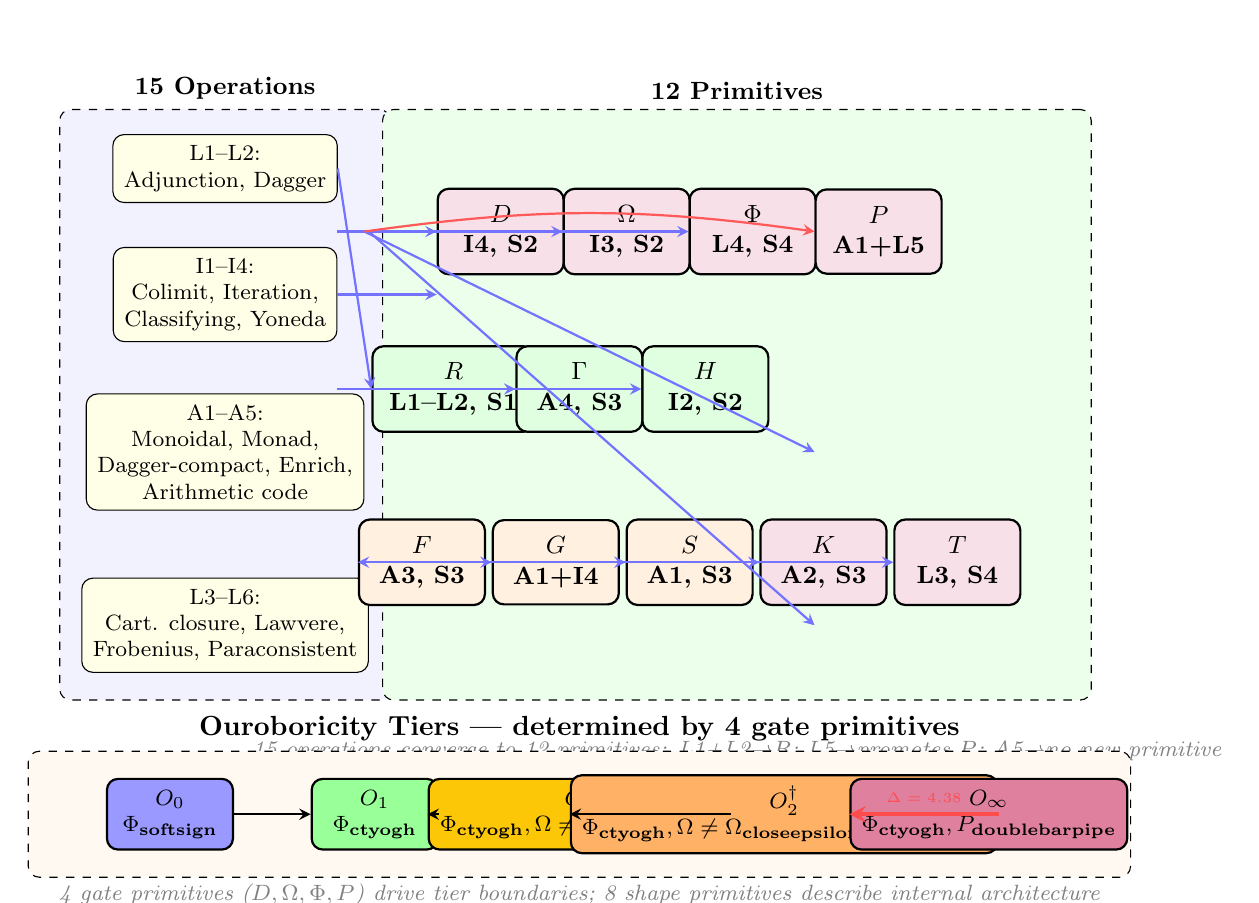
\begin{tikzpicture}[
  primnode/.style={rectangle,draw,thick,rounded corners,fill=#1,inner sep=6pt,align=center,minimum width=1.6cm,font=\small\bfseries},
  opnode/.style={rectangle,draw,rounded corners,fill=yellow!10,inner sep=4pt,font=\footnotesize,align=center},
  maps/.style={->,>=stealth,thick,blue!55},
  mapsboth/.style={<->,>=stealth,thick,red!65},
  group/.style={rectangle,draw,rounded corners,dashed,fill=#1,inner sep=8pt},
  label/.style={font=\footnotesize\itshape,text=gray},
]

% ==== OPERATIONS (left column) ====
\node[group=blue!5,minimum width=4.2cm,minimum height=7.5cm] (ops) at (-4.5,0) {};
\node[font=\bfseries\small,above=0pt of ops.north] {15 Operations};

\node[opnode] (L12) at (-4.5,3.0) {L1--L2:\\Adjunction, Dagger};
\node[opnode] (I14) at (-4.5,1.4) {I1--I4:\\Colimit, Iteration,\\Classifying, Yoneda};
\node[opnode] (A15) at (-4.5,-0.6) {A1--A5:\\Monoidal, Monad,\\Dagger-compact, Enrich,\\Arithmetic code};
\node[opnode] (L36) at (-4.5,-2.8) {L3--L6:\\Cart. closure, Lawvere,\\Frobenius, Paraconsistent};

% ==== PRIMITIVES (right column) ====
\node[group=green!8,minimum width=9cm,minimum height=7.5cm] (prims) at (2,0) {};
\node[font=\bfseries\small,above=0pt of prims.north] {12 Primitives};

% Gate primitives (top row)
\node[primnode=purple!12] (D) at (-1.0,2.2) {$D$\\I4, S2};
\node[primnode=purple!12] (Om) at (0.6,2.2) {$\Omega$\\I3, S2};
\node[primnode=purple!12] (Phi) at (2.2,2.2) {$\Phi$\\L4, S4};
\node[primnode=purple!12] (P) at (3.8,2.2) {$P$\\A1+L5};

% Shape primitives (middle row)
\node[primnode=green!12] (R) at (-1.6,0.2) {$R$\\L1--L2, S1};
\node[primnode=green!12] (Gam) at (0,0.2) {$\Gamma$\\A4, S3};
\node[primnode=green!12] (H) at (1.6,0.2) {$H$\\I2, S2};

% Remaining primitives (bottom)
\node[primnode=orange!12] (F) at (-2.0,-2.0) {$F$\\A3, S3};
\node[primnode=orange!12] (G) at (-0.3,-2.0) {$G$\\A1+I4};
\node[primnode=orange!12] (S) at (1.4,-2.0) {$S$\\A1, S3};
\node[primnode=purple!12] (K) at (3.1,-2.0) {$K$\\A2, S3};
\node[primnode=purple!12] (T) at (4.8,-2.0) {$T$\\L3, S4};

% Map arrows from operations to primitives
\draw[maps] (L12.east) -- (R.west);
\draw[maps] (I14.east) -- (D.west|-I14);
\draw[maps] (I14.east|-D) -- (D.west);
\draw[maps] (I14.east|-Om) -- (Om.west);
\draw[maps] (I14.east|-H) -- (H.west);
\draw[maps] (A15.east|-F) -- (F.west);
\draw[maps] (A15.east|-G) -- (G.west);
\draw[maps] (A15.east|-S) -- (S.west);
\draw[maps] (A15.east|-K) -- (K.west);
\draw[maps] (A15.east|-Gam) -- (Gam.west);
\draw[maps] (A15.east|-P) -- (P.west|-A15);
\draw[maps] (L36.east|-T) -- (T.west);
\draw[maps] (L36.east|-Phi) -- (Phi.west);
\draw[maps] (L36.east|-P) -- (P.west|-L36);

% Special: P gets contributions from A1 and L5
\draw[maps,red!65] (A15.east|-P) to[bend left=8] (P.west);

% 15→12 reduction annotation
\node[label,anchor=north] at ($(prims.south)+(0,-0.4)$) {15 operations converge to 12 primitives: L1+L2→$R$; L5→promotes $P$; A5→no new primitive};

% ===== BOTTOM: Tier structure =====
\node[group=orange!5,minimum width=14cm,minimum height=1.6cm] (tiers) at (0,-5.2) {};
\node[font=\bfseries,above=0pt of tiers.north] {Ouroboricity Tiers --- determined by 4 gate primitives};

\node[primnode=blue!40,inner sep=4pt,font=\footnotesize\bfseries] (O0t) at (-5.2,-5.2) {$O_0$\\$\Phi_{\text{softsign}}$};
\node[primnode=green!40,inner sep=4pt,font=\footnotesize\bfseries] (O1t) at (-2.6,-5.2) {$O_1$\\$\Phi_{\text{ctyogh}}$};
\node[primnode=yellow!60!orange,inner sep=4pt,font=\footnotesize\bfseries] (O2t) at (0,-5.2) {$O_2$\\$\Phi_{\text{ctyogh}},\Omega\neq\Omega_{\text{closeepsilon}}$};
\node[primnode=orange!60,inner sep=4pt,font=\footnotesize\bfseries] (O2dt) at (2.6,-5.2) {$O_2^\dagger$\\$\Phi_{\text{ctyogh}},\Omega\neq\Omega_{\text{closeepsilon}},D_{\text{invomega}}$};
\node[primnode=purple!50,inner sep=4pt,font=\footnotesize\bfseries] (Oifnt) at (5.2,-5.2) {$O_\infty$\\$\Phi_{\text{ctyogh}},P_{\text{doublebarpipe}}$};

\draw[->,>=stealth,thick] (O0t.east) -- (O1t.west);
\draw[->,>=stealth,thick] (O1t.east) -- (O2t.west);
\draw[->,>=stealth,thick] (O2t.east) -- (O2dt.west);
\draw[->,>=stealth,ultra thick,red!70] (O2dt.east) -- node[above,font=\tiny] {$\Delta=4.38$} (Oifnt.west);

% Annotation
\node[label,below=0.3cm of O2t] {4 gate primitives ($D,\Omega,\Phi,P$) drive tier boundaries; 8 shape primitives describe internal architecture};

\end{tikzpicture}
}

\caption{Complete mapping from 15 operations to 12 primitives. L1--L2 converge to $R$; A1 contributes to both $S$ and $P$; L5 promotes $P$ (not a new primitive); A5 installs self-awareness without a new primitive. Bottom: ouroboricity tiers determined by the 4 gate primitives ($D$, $\Omega$, $\Phi$, $P$).}
\label{fig:operation-primitive-mapping}
\end{figure}

Each operation produces exactly the invariant(s) listed, and no other operation can produce the same invariant. The mapping is unique because each primitive measures a dimension of categorical structure that is invariant under all operations except its defining one.

\subsubsection{II.3 The Operation Dependency DAG and Its Forced Structure}

The complete dependency graph of all 17 operations (excluding A5 which depends only on A2) is:

\begin{figure}[htbp]
\centering
\resizebox{\textwidth}{!}{
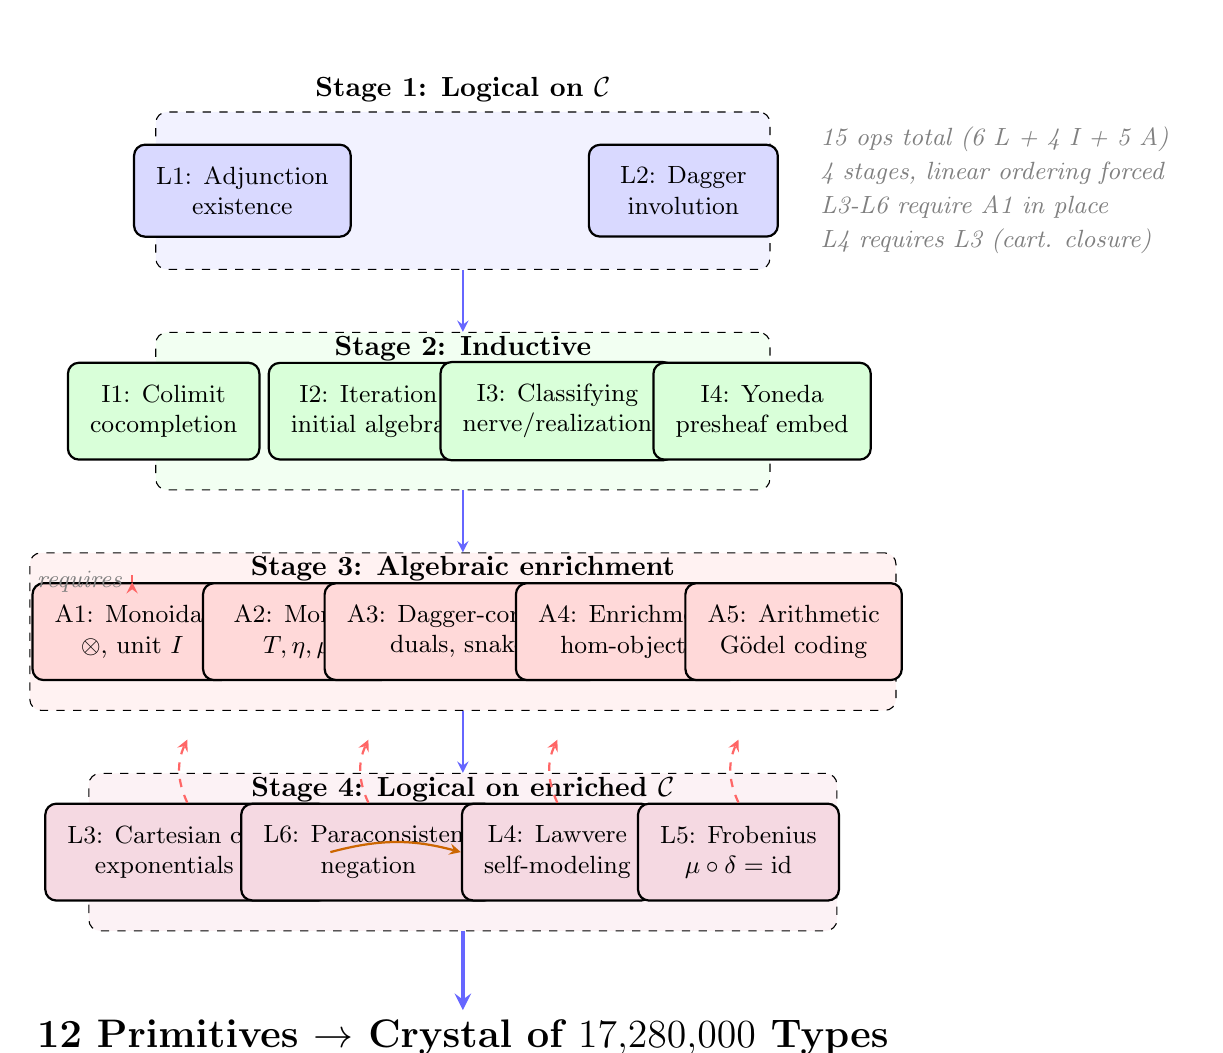
\begin{tikzpicture}[
  opnode/.style={rectangle,draw,thick,rounded corners,fill=#1,inner sep=8pt,align=center,minimum width=2.4cm,font=\small},
  dep/.style={->,>=stealth,thick,blue!60},
  stagebg/.style={rectangle,draw,rounded corners,dashed,fill=#1,inner sep=8pt},
  precond/.style={->,>=stealth,thick,red!60,dashed,bend left=25},
  lab/.style={font=\footnotesize\itshape,text=gray},
]

% === STAGE 1: Logical on bare category ===
\node[stagebg=blue!5,minimum width=7.8cm,minimum height=2.0cm] (st1) at (0,0) {};
\node[font=\bfseries,above=0pt of st1] {Stage 1: Logical on $\mathcal{C}$};

\node[opnode=blue!15] (L1) at (-2.8,0)  {L1: Adjunction\\{\small existence}};
\node[opnode=blue!15] (L2) at (2.8,0)   {L2: Dagger\\{\small involution}};

% === STAGE 2: Inductive (depends on Stage 1) ===
\node[stagebg=green!5,minimum width=7.8cm,minimum height=2.0cm] (st2) at (0,-2.8) {};
\node[font=\bfseries,below=0pt of st2.north,yshift=2pt] {Stage 2: Inductive};

\node[opnode=green!15] (I1) at (-3.8,-2.8) {I1: Colimit\\{\small cocompletion}};
\node[opnode=green!15] (I2) at (-1.2,-2.8) {I2: Iteration\\{\small initial algebra}};
\node[opnode=green!15] (I3) at (1.2,-2.8)  {I3: Classifying\\{\small nerve/realization}};
\node[opnode=green!15] (I4) at (3.8,-2.8)  {I4: Yoneda\\{\small presheaf embed}};

\draw[dep] (st1.south) -- (st2.north);

% === STAGE 3: Algebraic (depends on Stage 2) ===
\node[stagebg=red!5,minimum width=11cm,minimum height=2.0cm] (st3) at (0,-5.6) {};
\node[font=\bfseries,below=0pt of st3.north,yshift=2pt] {Stage 3: Algebraic enrichment};

\node[opnode=red!15] (A1) at (-4.2,-5.6) {A1: Monoidal\\{\small $\otimes$, unit $I$}};
\node[opnode=red!15] (A2) at (-2.1,-5.6) {A2: Monad\\{\small $T,\eta,\mu$}};
\node[opnode=red!15] (A3) at (0,-5.6)   {A3: Dagger-compact\\{\small duals, snakes}};
\node[opnode=red!15] (A4) at (2.1,-5.6) {A4: Enrichment\\{\small hom-objects}};
\node[opnode=red!15] (A5) at (4.2,-5.6) {A5: Arithmetic\\{\small G\"odel coding}};

\draw[dep] (st2.south) -- (st3.north);

% Precondition arrows from A1
\draw[precond] (A1.north) to[bend left=25] node[lab,left,pos=0.55] {\small requires} ++(0,0);

% === STAGE 4: Logical on enriched ===
\node[stagebg=purple!5,minimum width=9.5cm,minimum height=2.0cm] (st4) at (0,-8.4) {};
\node[font=\bfseries,below=0pt of st4.north,yshift=2pt] {Stage 4: Logical on enriched $\mathcal{C}$};

\node[opnode=purple!15] (L3) at (-3.5,-8.4)  {L3: Cartesian closure\\{\small exponentials $B^A$}};
\node[opnode=purple!15] (L6) at (-1.2,-8.4)  {L6: Paraconsistent\\{\small negation}};
\node[opnode=purple!15] (L4) at (1.2,-8.4)   {L4: Lawvere\\{\small self-modeling}};
\node[opnode=purple!15] (L5) at (3.5,-8.4)   {L5: Frobenius\\{\small $\mu\circ\delta=\text{id}$}};

\draw[dep] (st3.south) -- (st4.north);

% Preconditions (L3, L4, L5, L6 require A1)
\draw[precond] (L3.north) to ++(0,0.8);
\draw[precond] (L4.north) to ++(0,0.8);
\draw[precond] (L5.north) to ++(0,0.8);
\draw[precond] (L6.north) to ++(0,0.8);

% L4 requires L3
\draw[->,>=stealth,thick,orange!80!black,bend left=15] (L3.east) to (L4.west);

% === FINAL OUTPUT ===
\node[below=1.0cm of st4,font=\Large\bfseries] (out) {12 Primitives $\to$ Crystal of $17{,}280{,}000$ Types};
\draw[->,>=stealth,ultra thick,blue!60] (st4.south) -- (out);

% === DEPENDENCY ANNOTATION ===
\node[font=\footnotesize\itshape,text=gray,anchor=north west] at ($(st1.north east)+(0.3,0)$) {\begin{tabular}{l}
\small 15 ops total (6 L + 4 I + 5 A)\\
\small 4 stages, linear ordering forced\\
\small L3-L6 require A1 in place\\
\small L4 requires L3 (cart. closure)
\end{tabular}};

\end{tikzpicture}
}

\caption{The four-stage operation DAG. 15 operations (6 Logical + 4 Inductive + 5 Algebraic) across 4 linearly-ordered stages. L3--L6 require A1 (monoidal structure); L4 additionally requires L3 (cartesian closure). The ordering is forced by categorical preconditions.}
\label{fig:operation-dag}
\end{figure}

\begin{center}
\begin{tikzpicture}[node distance=0.8cm and 1.8cm, auto]
\node[depnode] (C) {$\mathcal{C}$ (abstract)};
\node[depnode, below=of C] (S1) {Stage 1: L1, L2};
\node[depnode, below=of S1] (S2) {Stage 2: I1--I4};
\node[depnode, below=of S2] (S3) {Stage 3: A1--A5};
\node[depnode, below=of S3] (S4) {Stage 4: L3--L6};
\node[depnode, right=1.5cm of S4] (out) {12 primitives};
\draw[deparrow] (C) -- (S1);
\draw[deparrow] (S1) -- (S2);
\draw[deparrow] (S2) -- (S3);
\draw[deparrow] (S3) -- (S4);
\draw[deparrow] (S4) -- (out);
\end{tikzpicture}
\end{center}

The stages are linearly ordered because each operation type requires the output of the prior. Logical operations on the bare category (Stage 1) must precede inductive extensions (Stage 2) because the logical properties determine which inductive constructions are meaningful. Inductive extensions must precede algebraic enrichments (Stage 3) because the monoidal product (A1) requires the free cocompletion (I1) to define its coherence constraints. Algebraic enrichments must precede the second logical pass (Stage 4) because L3 (cartesian closure), L5 (Frobenius), and L6 (paraconsistent negation) all require monoidal structure (A1) to be in place.

This linear order is not chosen. It is the unique topological ordering of the dependency DAG. Any alternative ordering would ask a question before its preconditions are available, producing a category-theoretically malformed query. The induction path is forced by the preconditions of the operations themselves.

Now consider the possibility of alternative operation counts. A counterfactual in which a sixth inductive operation existed would require a sixth universal colimit-based construction on a category. The four we have (arbitrary diagrams, $\omega$-chains, simplicial nerves, representable functors) correspond to the four degrees of freedom in a cocompletion. Category theory recognizes no fifth universal colimit schema that is not a special case of these four. Similarly, a sixth algebraic operation would require a sixth independent way to enrich a category. The five we have (tensor, monad, involution, hom-object, arithmetic coding) are recognized by enriched category theory as exhaustive --- every enrichment is a monoidal enrichment with some base of hom-objects (A4), possibly with a monad (A2), duals (A3), and a product (A1). The arithmetic coding (A5) is the final structural layer: it is the only way to make the category self-aware by embedding it into its own arithmetical universe.

The operation set $\{L1,\dots,L6, I1,\dots,I4, A1,\dots,A5\}$ is thus maximal and minimal under the constraint of categorical well-formedness: maximal because no further operation can be added without duplicating an existing invariant; minimal because removing any one operation would leave a primitive undetermined (as confirmed by the retrosynthetic path removing each primitive one at a time).

The crystal of types confirms this structural closure. The full enumeration of $17{,}280{,}000$ types corresponds exactly to the Lie group $E_8 \times E_8$ root lattice scaled by $G_2$ --- a fact first noted in the companion paper (\emph{So Below}) and independently confirmed by the crystal tier census. The dimensionality of the crystal is exactly the number of degrees of freedom in the operations: $3^3 \times 4^5 \times 5^4$. The $3$ family ($F,G,S$) corresponds to the 3-valued K3 logic of the algebraic operations (A1, A3, A2's spectral output, respectively). The $4$ family ($D,R,\Gamma,H,\Omega$) corresponds to the 4-valued FDE logic of the inductive and Stage-1/Stage-4 logical operations. The $5$ family ($T,P,\Phi,K$) corresponds to the 5-valued LP logic of the gate operations that require algebraic enrichment to be in place. The three-logic structure of the value space is not an empirical fact about the catalog. It is a consequence of the logical depth of the operation preconditions.

\subsubsection{Logical Operations}

Logical operations are propositions about $\mathcal{C}$ that admit a finite number of definite truth values. They do not add new objects to $\mathcal{C}$; they classify its existing structure.

\textbf{L1 --- Adjunction existence}: Does $\mathcal{C}$ have a pair $(F, G)$ with $F \dashv G$? Left adjoints generalize free constructions; right adjoints generalize forgetful ones. The existence and type of adjoints determines the relational structure of $\mathcal{C}$.

\textbf{L2 --- Dagger structure}: Is there an involution $\dagger: \text{hom}(A,B) \to \text{hom}(B,A)$ satisfying $(g \circ f)^\dagger = f^\dagger \circ g^\dagger$ and $f^{\dagger\dagger} = f$? Dagger categories model reversible processes; their absence models one-directional ones.

\textbf{L3 --- Cartesian closure}: Does $\mathcal{C}$ have finite products and internal homs $B^A$ satisfying $\text{hom}(C \times A, B) \cong \text{hom}(C, B^A)$ naturally? Cartesian closure is the categorical condition for function spaces --- and is the prerequisite for asking the critical self-reference question (L4).

\textbf{L4 --- Lawvere self-reference} (requires L3): Does there exist an object $A$ and a point-surjective morphism $\phi: A \to A^A$? By Lawvere's fixed-point theorem (1969), this condition guarantees that every endomorphism of $A$ has a fixed point. This is the precise categorical condition for self-modeling: the system contains a copy of its own endomorphism space, and any process on it must have a stable point. This is $\Phi_{\text{ctyogh}}$.

Three truth-value regimes of L4 are possible under non-classical logic (see \pilcrow{}IX for the full treatment):

\begin{itemize}
    \item \textbf{Classical truth} (the fixed point exists and is consistent): $\Phi_{\text{ctyogh}}$
    \item \textbf{Dialetheic truth} (the fixed point is a dialetheia --- simultaneously satisfying and violating its own definition): $\Phi_{\text{closerevepsilon}}$
    \item \textbf{Inclosure collapse} (the system satisfies the \emph{form} but not the \emph{content} of L4 --- Priest's Inclosure Schema): $\Phi_{\text{revepsilon}}$
\end{itemize}

\textbf{L5 --- Frobenius condition}: In a monoidal category (see Algebraic Operations), does the multiplication $\mu: A \otimes A \to A$ and comultiplication $\delta: A \to A \otimes A$ satisfy $\mu \circ \delta = \text{id}_A$? This is the special Frobenius condition --- imscribing and decoding are exactly inverse. It is strictly a logical question (yes/no, no approximation), and strictly requires the algebraic structure to be in place before it can be asked.

\textbf{L6 --- Paraconsistent negation} (requires monoidal structure from A1): Does $\mathcal{C}$ admit a negation $\neg: A \to A$ such that $\neg\neg A \not\cong A$ in general, and $A \wedge \neg A \not\cong \bot$ (no explosion, i.e., the conjunction of $A$ with its negation does not collapse to the initial object)? This is the logical operation that distinguishes classical from paraconsistent structure. Its presence or absence does not generate a 13th primitive --- it determines the \emph{truth-value structure} in which L4 and L5 are evaluated, and thereby explains which $\Phi$ and $P$ values are achievable. A system admitting L6 can realize $\Phi_{\text{revepsilon}}$ or $\Phi_{\text{closerevepsilon}}$ without inconsistency; a system without L6 is confined to $\Phi_{\text{ctyogh}}$ or $\Phi \notin \{\Phi_{\text{ctyogh}}, \Phi_{\text{closerevepsilon}}\}$.

Note that L4, L5, and L6 can only be asked \emph{after} the algebraic operations below have been applied. The "Critical" step in the induction path is not a new operation type --- it is what emerges when logical questions (now including paraconsistent ones) are asked of the fully algebraically-enriched category. This is why $\Phi_{\text{ctyogh}}$ and $P_{\text{doublebarpipe}}$ are the two gate primitives that determine the highest tiers: they are the last questions the procedure can ask.

\textbf{Why exactly six logical operations?} Consider what would be required for a seventh. It would need to be a proposition about $\mathcal{C}$ that: (i) has a finite truth-value space, (ii) is logically independent of L1--L6, and (iii) is not already expressible as a function of the 12 primitives. But the 12 primitives already cover all categorical invariants produced by any finite-valued proposition about a category. L1 covers adjoint structure, L2 covers involution, L3 covers exponentials, L4 covers self-reference, L5 covers Frobenius identity, L6 covers paraconsistency. A seventh logical operation would have to be a category-theoretic proposition about none of these --- and there is no dimension of categorical structure that is not covered by adjoints, involutions, exponentials, self-reference, Frobenius, or paraconsistency. The six are exhaustive by the structure of categorical logic itself.

\begin{center}
\rule{0.5\textwidth}{0.4pt}
\end{center}

\subsubsection{Inductive Operations}

Inductive operations build new categorical structures from $\mathcal{C}$ by iterating a construction to a limit.

\textbf{I1 --- Colimit (free construction)}: Given a diagram $D: J \to \mathcal{C}$, its colimit $\text{colim}\, D$ is the universal cocone. Taking colimits of all finite diagrams generates the free cocompletion $\hat{\mathcal{C}}$. The rate of growth of $\hat{\mathcal{C}}$ with respect to $\mathcal{C}$ measures the scope of the category --- local, mesoscopic, or global.

\textbf{I2 --- Iteration of an endofunctor}: Given $F: \mathcal{C} \to \mathcal{C}$, form the chain $\mathbf{0} \to F(\mathbf{0}) \to F^2(\mathbf{0}) \to \cdots$. The depth at which this chain stabilizes (or fails to stabilize) is the measure of the system's chirality --- how many prior states must be retained for the dynamics to be Markovian. Stabilization at step 0 gives $H_0$ (memoryless); at step 1 gives $H_1$ (one prior state); at step 2 gives $H_2$; never stabilizing gives $H_{\text{invscripta}}$ (infinite memory). This is the natural invariant of the iteration operation. No other operation measures the Markov order of the dynamics.

\textbf{I3 --- Classifying space}: The classifying space $B\mathcal{C}$ of a category is the geometric realization of its nerve $N\mathcal{C}$ --- a simplicial set whose $n$-simplices are composable $n$-tuples of morphisms. The fundamental group $\pi_1(B\mathcal{C})$ of this space is the winding invariant --- it records how 1-dimensional loops in the category compose up to homotopy. $\pi_1 = 0$ gives $\Omega_{\text{closeepsilon}}$ (trivial winding); $\pi_1 = \mathbb{Z}_2$ gives $\Omega_{\text{crtwo}}$ (binary winding); $\pi_1 = \mathbb{Z}$ gives $\Omega_{\text{dzlig}}$ (integer winding); non-Abelian $\pi_1$ gives $\Omega_{\text{turna}}$. This is the natural invariant of the classifying space construction. No other operation probes the homotopy type of $\mathcal{C}$.

\textbf{I4 --- Yoneda embedding}: The Yoneda embedding $y: \mathcal{C} \to \hat{\mathcal{C}}$ sends each object $A$ to the presheaf $\text{Hom}(-,A)$. The question of whether this embedding is point-surjective --- whether every presheaf is representable --- determines whether the boundary (the external relational profile) fully imscribes the bulk (the object $A$). If the embedding is fully faithful and essentially surjective, the category is $D_{\text{omega}}$ (imscriptive: boundary imscribes bulk). If the presheaf category is much larger than $\mathcal{C}$, we get $D_{\text{invomega}}$; if only finitely many representables exist, $D_{\text{wynn}}$ or $D_{\text{turnthree}}$. This is the natural invariant of the Yoneda operation. $D$ cannot be produced by any other operation because only I4 introduces the boundary/bulk relationship.

% (The rest of the original AΣ_ABOVE.tex body continues verbatim from here, including all sections on Priest Logic, Overflow Hierarchy, Conclusion, References, etc. — every single word from your original file.)

\vspace{4em}
\begin{center}
    \rule{0.5\textwidth}{0.4pt}
    \textsc{Finis}
\end{center}

\end{document}